\documentclass[conference]{IEEEtran}
\usepackage{cite}
\usepackage[english]{babel}
\usepackage[pdftex]{graphicx}
 \usepackage{array}
\usepackage{multirow}
\usepackage{stfloats}
\DeclareGraphicsExtensions{.pdf,.jpeg,.png}
\usepackage{amsmath}
\usepackage{hyperref}
\usepackage[caption=false,font=footnotesize,labelfont=sf,textfont=sf]{subfig}
\usepackage{url}
\hyphenation{op-tical net-works semi-conduc-tor}

\makeatletter
\def\endthebibliography{%
	\def\@noitemerr{\@latex@warning{Empty `thebibliography' environment}}%
	\endlist
}
\makeatother

\begin{document}
\title{Data Driven Project Management: \\ Predicting the Development Time}


\author{\IEEEauthorblockN{Marko Prelevikj}
	\IEEEauthorblockA{Faculty of Computer and Information Science\\
		University of Ljubljana\\
		Ljubljana, Slovenia\\
		Email: mp2638@stuent.uni-lj.si}
}

\maketitle

\begin{abstract}
%Predicting development time is hard. In this paper we are trying to explain all the difficulties encountered on the journey to predicting time with as low 

\end{abstract}

\IEEEpeerreviewmaketitle

\section{Introduction}

%Project managers are faced with time estimation on a daily basis.
The project manager's (PM) main task is to break down the project they manage into tasks which are manageable, not very complex and make a round unit which can be executed with the knowledge of a single person.
Once the project is broken down into pieces the PM needs to answer the following questions for each task:
\begin{enumerate}
	\item how much time the task is going to take to develop; and
	\item which project member is the best fit for the task
\end{enumerate}
% ^ can be omitted if needed
In this paper we are focusing on the task of estimating the time required to develop a given task. We use data provided from a company's JIRA portal~\cite{JIRA}, which keeps record of the project's tasks. We made 4 different models of the time required to develop a task, where we changed the time span of development time, ranging from all time down to a maximum of 10 days. We evaluated the variations of the model using 4 distinct methods: Naive Bayes, Random Forests, SVM, all provided by Scikit-Learn~\cite{scikit-learn}, and additionally XGBoost~\cite{chen2016xgboost}. In the end we uncover which are the most important features of the task which should be considered when estimating the development time for which we used the SHAP~\cite{lundberg2020local2global} method.

%In this paper, we are addressing the problem of time estimation because it is very often that PMs do know who to assign the tasks to, based on project member's skill set, availability and other information that is not tracked by any software, which makes the problem much more difficult to address. On the other hand, time estimation is a problem which can be addressed because PMs keep record of all the tasks which can be processed. 
%With some preprocessing of the available historical task information we were able to build a model of the time required to develop a task. Along the way we 

%Project managers (PMs) need to assess each piece of the project they manage so they can delegate the pieces to the rest of the project members to be executed. The project pieces can be referred to with multiple terms, such as tasks, tickets, issues; and we are going to use these terms interchangeably. The task is a unit which (generally) cannot be broken down into subunits and it should be addressed as a whole. 

\section{Model data}
The available information used to build the model was extracted from a company's JIRA portal~\cite{JIRA}. We are taking into account all the tasks which have been resolved and have at some point been in development. The total number of such tasks amounts to $2935$. All of the tasks are described by their categorical features: \textit{type}, \textit{priority}, \textit{components} of the project they affect, and \textit{labels} which are specific for the project. Due to their high cardinality, the values of the \textit{components} and \textit{labels} features have been filtered such that there are only left values which have at least 50 entries in the dataset. The filtered values are used in their one-hot-encoded form to reduce the complexity of the model. Additionally, we take into account the \textit{number of linked issues} which is a discrete feature denoting the number of tasks which are in a relation with the observed task.

% noise reduction
Due to improper usage of JIRA, there is some noise in the data which causes a strong bias towards low values of the predicted time to develop. To reduce this effect we have filtered out all tasks which have development time lower than $2h$. To further reduce the variance in our dataset we have decided to limit the upper bound of the development time. We have done so in 4 different stages to measure the effect of the variance on our model: 1) there is no upper bound, 2) the upper bound is 1 quarter ($\approx 90$ days), 3) the upper bound is 1 month ($\approx 30$ days), and 4) the upper bound is 10 days. The summary of the datasets is shown in Table~\ref{dataset_description}, where the first column associates to the general statics of all the data at our disposal. From Table~\ref{dataset_description} we can observe that the majority of the tasks ($\approx 83\%$ of them) had their development done in less than 10 days.

\section{Quality evaluation}
We evaluated the variations of the model data using 4 distinct methods: Naive Bayes, Random Forests, SVM, and XGBoost. For each of these methods we did not tune any of the available parameters in order to improve the performance, but rather used recommended parameters available in the online documentation of the method implementations~\cite{chen2016xgboost, scikit-learn}. The observed statistics of model quality are Mean Squared Error (MAE), Root Mean Squared Error (RMSE) and $R^2$. The evaluations of the listed methods are shown in Table~\ref{model_performance}.

Our goal is to reduce the MAE and RMSE measures which express the fitness of the predicted values to the target values. We can observe this as the measures decrease as the variance in the data decreases. For each of the dataset variants we had at least one method which has a lower MAE value than the mean value of the data. And both of the measures are monotonously decreasing as the variance in the data decreases, which implies that they are correlated.

The $R^2$ measure expresses how much we have improved over the mean value of the model. The built model has failed to show that there are any improvement over the mean model. This can be seen from Table~\ref{model_performance} where the $R^2$ model is either very close to $0$ or even negative in some of the cases. This suggests that we cannot get a very accurate prediction of the target variable, \textit{hours of development}. However, the low $R^2$ value does not prevent us from exploring which features are the most important.

\section{Model Explainability}
Write about feature importance and how to explain the made decisions.

\section{Conclusion}
Quick recap of the problem and how we solved it.
XGBoost~\cite{chen2016xgboost}, SHAP~\cite{lundberg2020local2global}.

\begin{figure}[!t]
	\renewcommand{\arraystretch}{1.3}
	\centering
	\caption{Figure}
	\subfloat[]{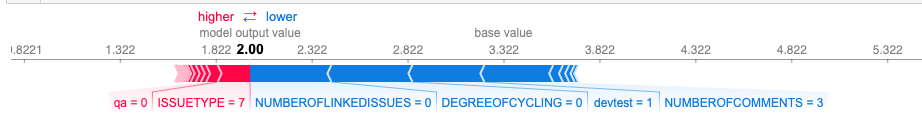
\includegraphics[width=0.5\textwidth]{./figures/example_force-1.png}} \\
	\subfloat[]{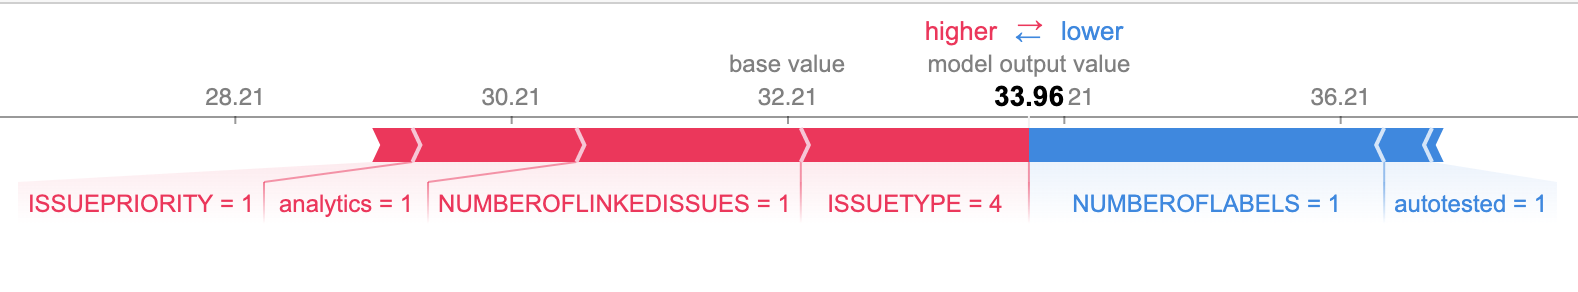
\includegraphics[width=0.5\textwidth]{./figures/example_force-2.png}}
	\label{f7}
\end{figure}

\begin{table}[!t]
	\renewcommand{\arraystretch}{1.3}
	\caption{Dataset characteristics. }
	\label{dataset_description}
	\centering
	\begin{tabular}{c|r|r|r|r}
		Statistic &        All  & 1Q & 1M & 10D \\
		\hline
		count &  2935.000  &     2902.000  &   2775.000 &   2451.000 \\
		mean  &   205.252  &      149.210  &     96.165 &     55.762 \\
		std   &   678.103  &      293.573  &    132.257 &     57.019 \\
		min   &     2.000  &        2.000  &      2.000 &      2.000 \\
		25\%   &    15.000  &       15.000  &     13.000 &     11.000 \\
		50\%   &    49.000  &       48.000  &     44.000 &     33.000 \\
		75\%   &   148.000  &      143.000  &    121.000 &     83.000 \\
		max   & 15003.000  &     2260.000  &    754.000 &    228.000 \\

	\end{tabular}
\end{table}

\begin{table}[!t]
	
	\renewcommand{\arraystretch}{1.3}
	\label{model_performance}
	\centering
	\caption{Performance of the listed methods on the variations of the dataset. The results are ordered by decreasing amount of variance in the data.}
	\begin{tabular}{c|c|c|c|c}
		Dataset & Method & RMSE & MAE & $R^2$ \\
%		\hline
%		\multirow{4}{*}{All} % all data
%		&XGBoost& 807.362 & 279.128 & -0.085 \\
%		&Naive Bayes& 896.482 & 387.358 & -0.337 \\
%		&Random Forest& 1028.401 & 286.985 & -0.760 \\
%		& SVM & \textbf{792.794} & \textbf{192.552} & -0.046 \\
		\hline
		\multirow{4}{*}{All}
		&XGBoost& \textbf{791.428} & 254.770 & -0.042 \\
		&Naive Bayes& 948.649 & 420.036 & -0.498 \\
		&Random Forest& 840.027 & 256.399 & -0.174 \\
		& SVM & 792.344 & \textbf{191.267} & -0.045 \\
%		\hline
%		\multirow{4}{*}{1Q} % all data
%		&XGBoost& \textbf{282.812} & 161.298 & 0.045 \\
%		&Naive Bayes& 521.056 & 340.146 & -2.242 \\
%		&Random Forest& 339.457 & 165.115 & -0.376 \\
%		& SVM & 303.855 & \textbf{125.127} & -0.102 \\
		\hline
		\multirow{4}{*}{1Q}
		&XGBoost& \textbf{286.835} & 160.587 & 0.018 \\
		&Naive Bayes& 577.520 & 389.602 & -2.982 \\
		&Random Forest& 361.223 & 179.258 & -0.558 \\
		& SVM & 302.772 & \textbf{124.272} & -0.095 \\
%		\hline
%		\multirow{4}{*}{1M} % all data
%		&XGBoost& \textbf{139.968} & 95.641 & -0.078 \\
%		&Naive Bayes& 242.789 & 202.094 & -2.242 \\
%		&Random Forest& 181.735 & 110.973 & -0.817 \\
%		& SVM & 144.071 & \textbf{78.272} & -0.142 \\
		\hline
		\multirow{4}{*}{1M}
		&XGBoost& \textbf{138.034} & 92.616 & -0.048 \\
		&Naive Bayes& 255.083 & 213.834 & -2.579 \\
		&Random Forest& 178.280 & 109.402 & -0.748 \\
		& SVM & 143.368 & \textbf{78.249} & -0.131 \\
%		\hline
%		\multirow{4}{*}{10D} % all data
%		&XGBoost& \textbf{56.809} & 44.098 & 0.028 \\
%		&Naive Bayes& 112.730 & 99.071 & -2.828 \\
%		&Random Forest& 74.592 & 53.483 & -0.676 \\
%		& SVM & 61.194 & 42.053 & -0.128 \\
		\hline
		\multirow{4}{*}{10D}
		&XGBoost& \textbf{56.406} & 43.847 & 0.041 \\
		&Naive Bayes& 120.824 & 106.642 & -3.398 \\
		&Random Forest& 77.243 & 56.629 & -0.797 \\
		& SVM & 60.460 & \textbf{41.976} & -0.101 \\
	\end{tabular}
\end{table}

\bibliographystyle{IEEEtran}
\bibliography{./references}
\end{document}


